\subsection{Sequence}

I \textbf{diagrammi di sequenza} appartengono alla categoria dei diagrammi di interazione, i quali descrivono la collaborazione di un gruppo di oggetti che devono implementare un certo comportamento. Un diagramma di sequenza documenta tipicamente il comportamento di un singolo scenario. Il diagramma include un certo numero di oggetti e i messaggi scambiati tra essi durante l’esecuzione del caso d’uso.

\paragraph{Esempio: calcolo del prezzo di un ordine}
L’ordine deve calcolare il prezzo di ciascuna linea. Per farlo, occorre ottenere la quantità relativa al prodotto e il suo prezzo unitario. Una volta calcolato il prezzo totale, si calcola lo sconto che dipende dallo specifico cliente. Queste interazioni sono illustrate nel diagramma di sequenza riportato di seguito.

\begin{figure}[H]
    \centering
    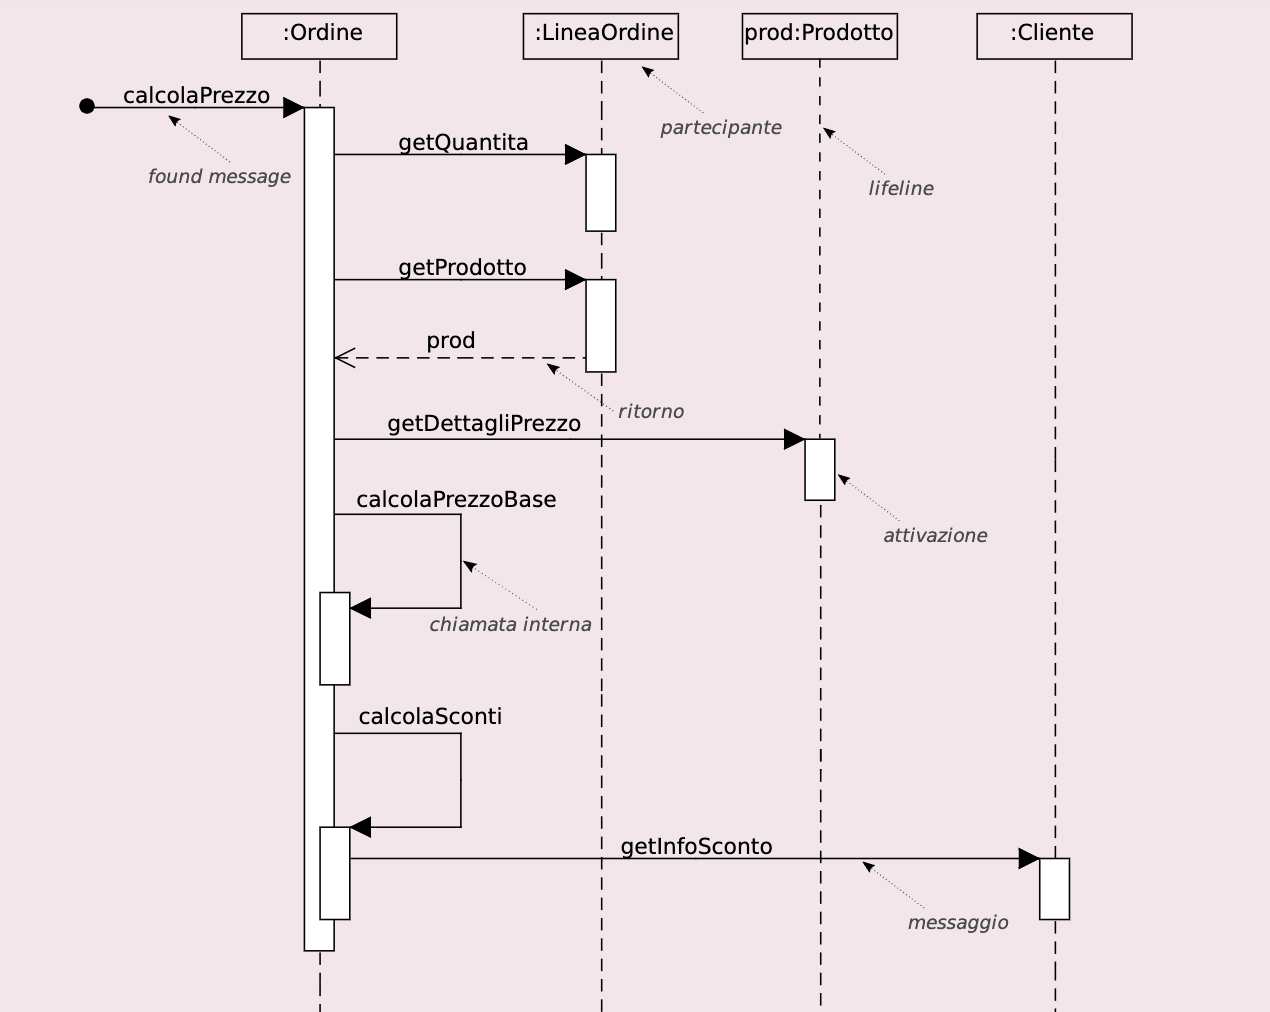
\includegraphics[width=0.75\linewidth]{assets/UML/sequence/sequence-1.png}
    \caption{Diagramma di sequenza a controllo centralizzato}
\end{figure}

\paragraph{Elementi di un diagramma di sequenza}
Ciascun partecipante è rappresentato da un box che contiene il nome (nella notazione degli Object Diagram, ma non sottolineato) e da una linea tratteggiata verticale detta \textbf{linea di vita} (\textit{lifeline}). L’ordinamento dei messaggi è determinato scorrendo il diagramma dall’alto verso il basso. Ogni linea di vita ha una barra di attivazione che indica quando il partecipante è attivo nell’interazione. Le frecce indicano i messaggi (invocazioni) e sono etichettate con il nome del messaggio (nome del metodo). Le frecce di ritorno sono opzionali e possono riportare il valore risultante dall’invocazione.

\paragraph{Controllo centralizzato e controllo distribuito}
Esistono due stili principali di interazione:
\begin{itemize}
    \item \textbf{Controllo centralizzato}: un partecipante svolge tutta l’interazione, gli altri forniscono solo i dati.
    \item \textbf{Controllo distribuito}: i compiti sono ripartiti tra i partecipanti, sfruttando il polimorfismo e la logica distribuita.
\end{itemize}

\begin{figure}[H]
    \centering
    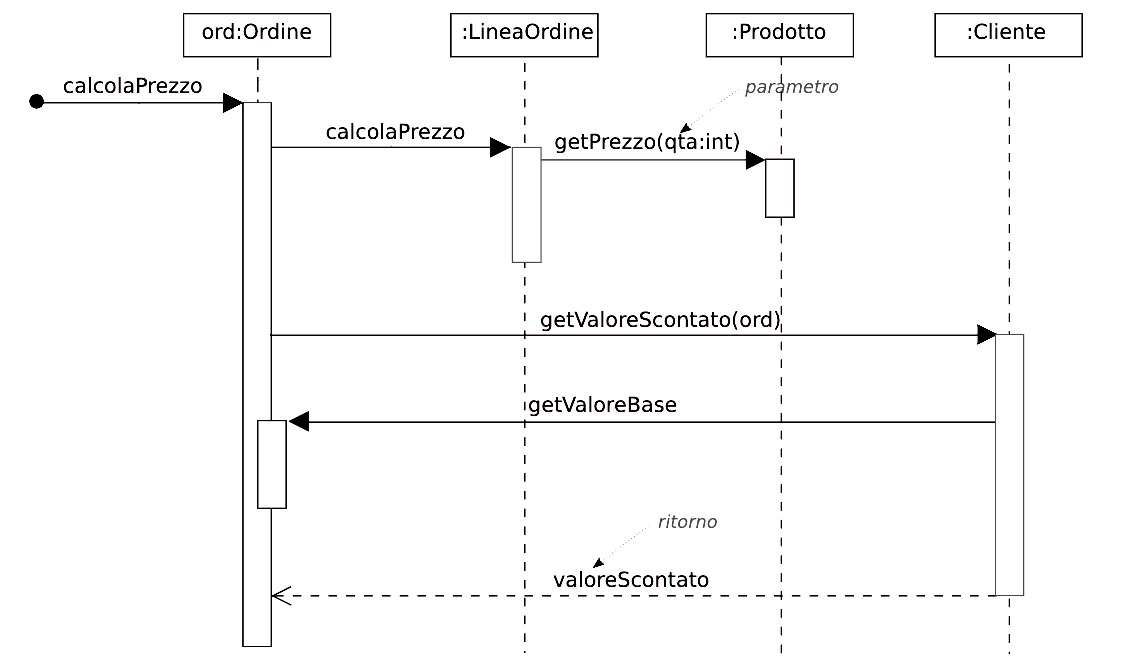
\includegraphics[width=0.75\linewidth]{assets/UML/sequence/sequence-2.png}
    \caption{Diagramma di sequenza a controllo distribuito}
\end{figure}

\paragraph{Creazione e distruzione dei partecipanti}
I diagrammi di sequenza prevedono una notazione particolare per indicare la creazione e la distruzione dei partecipanti:
\begin{itemize}
    \item \textbf{Creazione}: la freccia del messaggio che causa la creazione punta al box del partecipante creato.
    \item \textbf{Distruzione}: indicata con una \textbf{X} posizionata sulla linea di vita. Può essere causata da un altro oggetto o essere autodistruzione.
\end{itemize}

\begin{figure}[H]
    \centering
    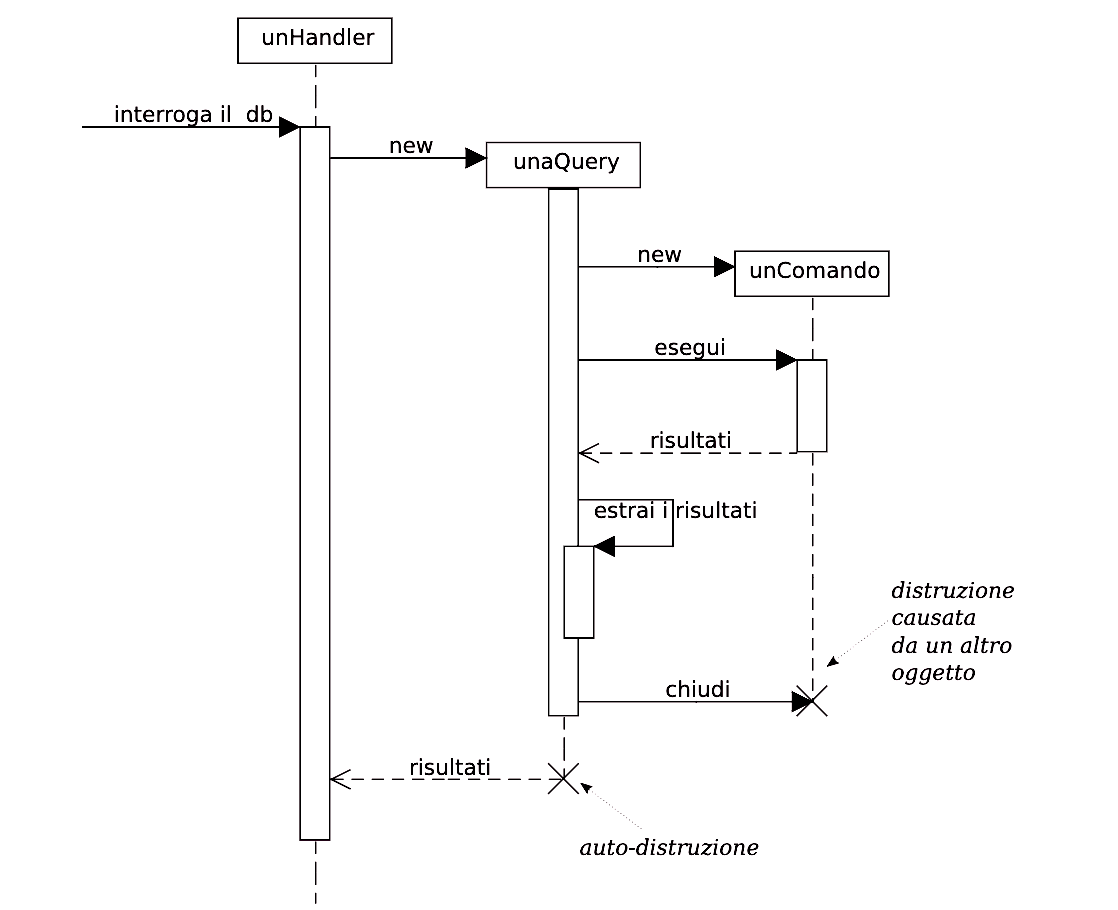
\includegraphics[width=0.75\linewidth]{assets/UML/sequence/sequence-3.png}
    \caption{Creazione e distruzione dei partecipanti}
\end{figure}

\paragraph{Frame di interazione}
Per rappresentare comportamenti ciclici e/o condizionali, si utilizzano i \textbf{frame di interazione}, cornici che includono uno o più frammenti di diagramma. Ogni frame ha un operatore e ogni frammento può avere una guardia.

\begin{table}[H]
    \centering
    \begin{tabularx}{\textwidth}{|l|X|}
        \hline
        \textbf{Operatore} & \textbf{Significato} \\
        \hline
        \textbf{alt} & Frammenti multipli in alternativa; si esegue solo quello per cui la condizione è soddisfatta. \\
        \hline
        \textbf{opt} & Opzionale; il frammento è eseguito solo se la condizione è verificata. \\
        \hline
        \textbf{par} & Parallelo; ogni frammento è eseguito in parallelo. \\
        \hline
        \textbf{loop} & Ciclo; il frammento può essere eseguito più volte, la guardia indica la condizione di iterazione. \\
        \hline
        \textbf{region} & Regione critica; il frammento può essere eseguito da un solo thread alla volta. \\
        \hline
        \textbf{neg} & Negativo; il frammento mostra un’interazione non valida. \\
        \hline
        \textbf{ref} & Riferimento; si riferisce a un’interazione mostrata in un altro diagramma. \\
        \hline
        \textbf{sd} & Sequence Diagram; usato per racchiudere un intero diagramma di sequenza. \\
        \hline
    \end{tabularx}
    \caption{Operatori dei frame di interazione}
\end{table}

\begin{figure}[H]
    \centering
    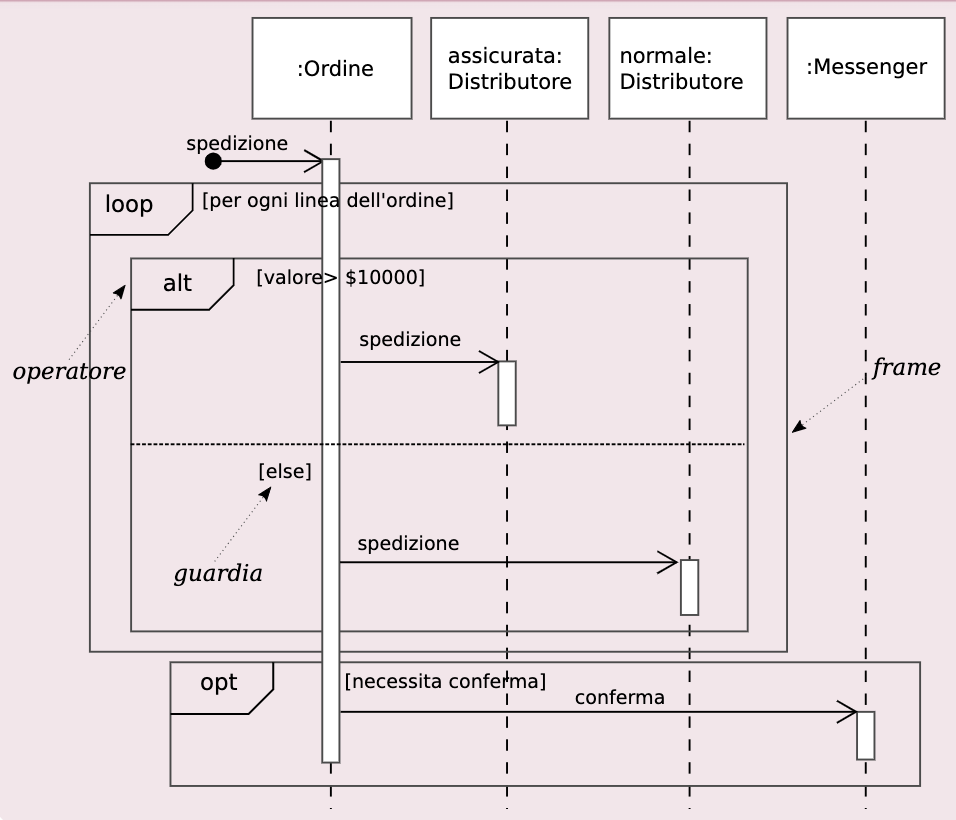
\includegraphics[width=0.75\linewidth]{assets/UML/sequence/sequence-4.png}
    \caption{Esempio di frame di interazione}
\end{figure}

\paragraph{Chiamate sincrone e asincrone}
UML distingue i messaggi sincroni dai messaggi asincroni tramite il tipo di freccia utilizzata:
\begin{itemize}
    \item \textbf{Messaggi sincroni}: freccia con punta a forma di triangolo pieno. L’oggetto che invia il messaggio deve attendere la risposta prima di proseguire.
    \item \textbf{Messaggi asincroni}: freccia con punta costituita da due linee sottili. Utilizzati nelle applicazioni multi-thread o distribuite.
\end{itemize}

\newpage